\documentclass[12pt]{article}
\usepackage{fullpage}
\usepackage{nopageno}
\usepackage{ifthen}
\usepackage{amsmath}
\usepackage{amssymb}
\usepackage{graphicx} 
\usepackage{version}
\usepackage{amsthm}
\usepackage{multicol}
\usepackage{add-copyright}

\excludeversion{solution}

\DeclareMathOperator{\ft}{ft}

\newcommand{\R}{\mathbb{R}}

\title{Take-Home Quiz 6}
\author{Math 132 Section 22}
\date{Due Wednesday, March 8, 2006}

\newcounter{problem}
\setcounter{problem}{1}

\newenvironment{problem}[1][]
{\begin{flushleft}\hangindent=1em\hangafter=1\noindent\textbf{Problem \arabic{problem}.}
\ifthenelse{\equal{#1}{}}{}{
\textbf{(#1 \ifthenelse{\equal{#1}{1}}{point}{points}).}}
}
{\addtocounter{problem}{1}\end{flushleft}}

\begin{document}
\maketitle

\begin{problem}[3]
  Find the volume of a ball of radius~$r$ with a hole of radius~$a$
  drilled through it.  Specifically, find the volume of
  $$
  \{ (x,y,z) \in \R^3 : \sqrt{x^2 + y^2 + z^2} \leq r \mbox{ and } \sqrt{x^2 + y^2} \geq a \}.
  $$
  The first condition (i.e., $\sqrt{x^2 + y^2 + z^2}$) picks out those
  points which are inside the ball of radius $r$, and the second
  condition (i.e., $\sqrt{x^2 + y^2} \geq a$) picks out those points
  which are outside a cylinder of radius $a$.  \textit{Hint:} use the
  method of shells.
\end{problem}

\begin{problem}[3]
  Find the length of the curve defined for $0 \leq t \leq 4$ by
  \begin{eqnarray*}
    x(t) &=& t, \\
    y(t) &=& \frac{2 t^{3/2}}{3}.
  \end{eqnarray*}
\end{problem}

\begin{problem}[4]
  Where is the center of mass of a hemisphere of radius~1?
\end{problem}

\begin{problem}[4]
  Archimedes, in a recently discovered book called \textit{The
  Method}, describes a procedure for computing the volume of a sphere.
  He begins by building a mobile, with a cylinder of height~$r$ and
  radius~$r$ on one side balanced against a hemisphere of radius~$r$
  and a cone of radius~$r$ and height~$r$ on the other side:
\begin{center}
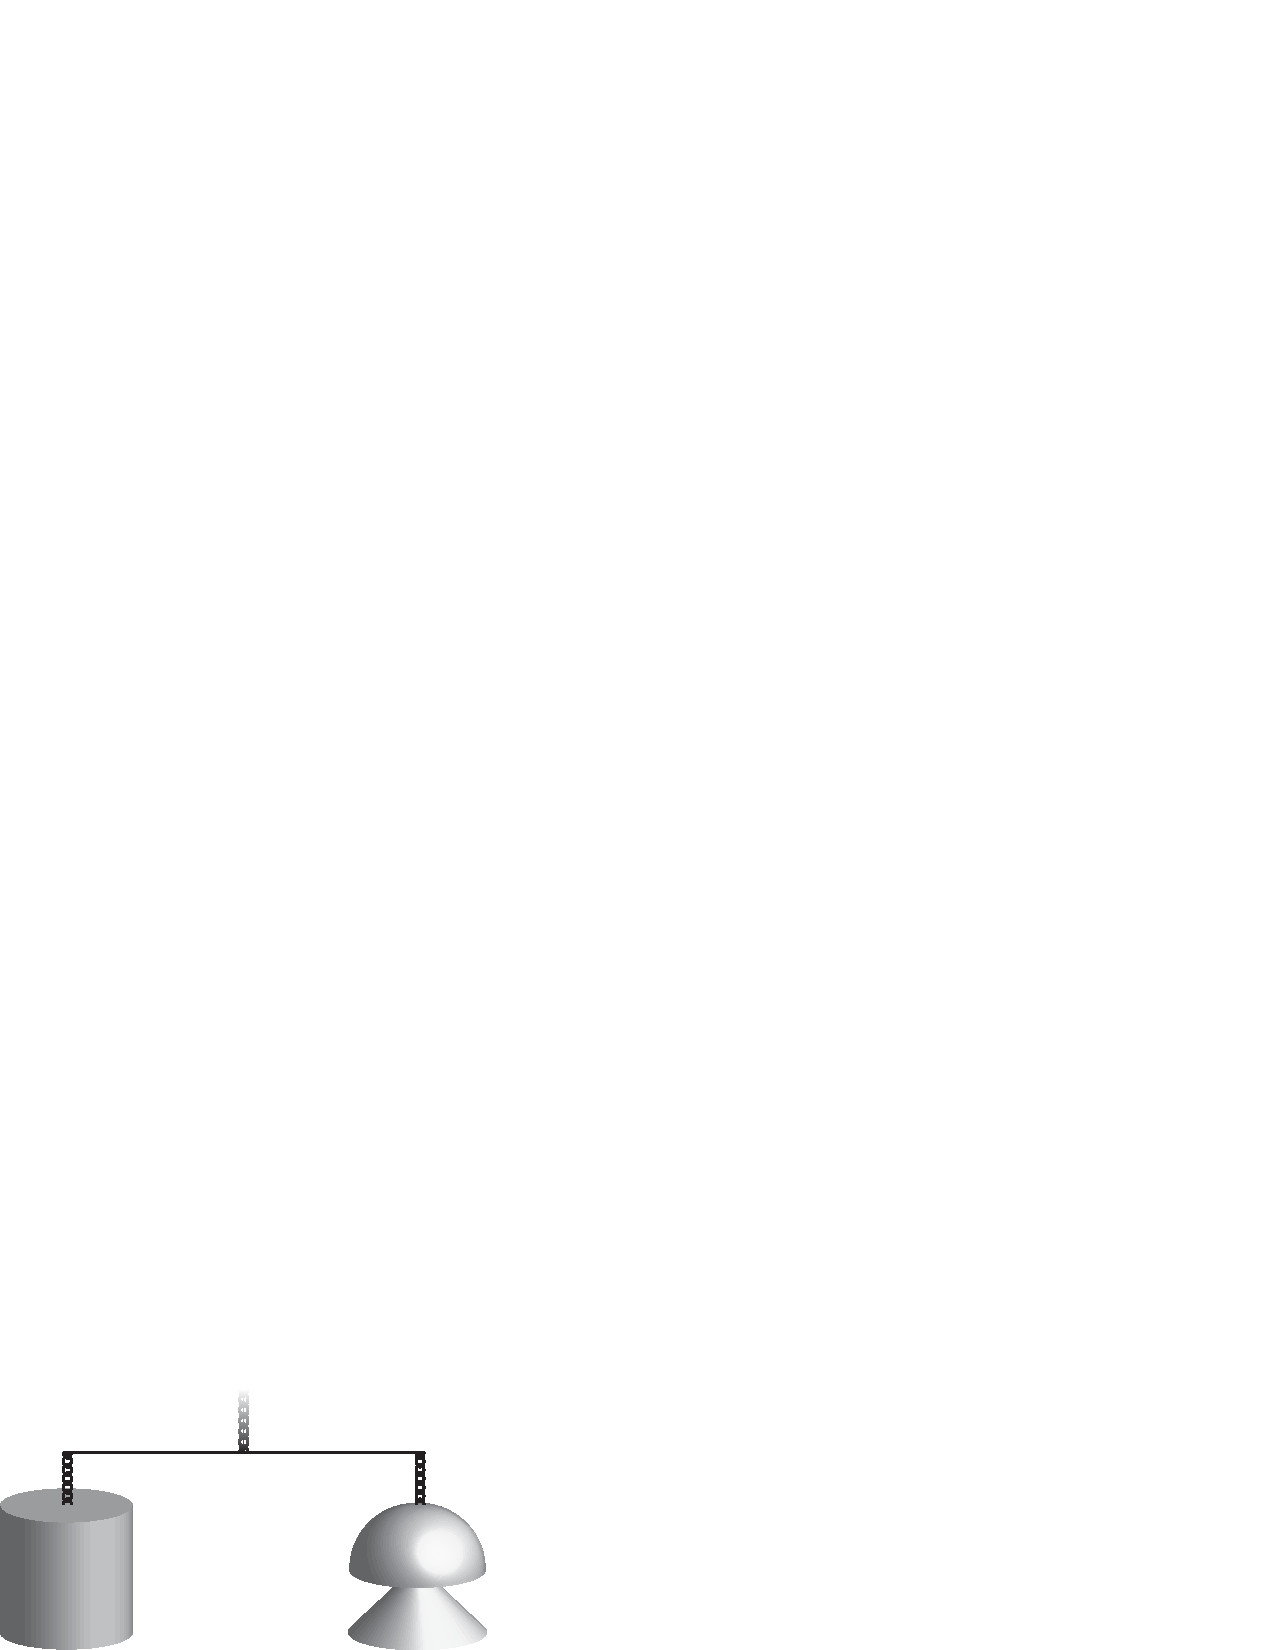
\includegraphics{archimedes.pdf}
\end{center}
You may assume that the volume of the cylinder is $\pi r^3$, and that
the volume of the cone is $\pi r^3/3$, and that the balance point is
at the midpoint.  Explain why the mobile balances and therefore prove
that the volume of a hemisphere is $2 \pi r^3/3$.
\end{problem}


%\begin{problem}[3]
%There is a spring attached to the wall; unable to resist, you pull the
%free end, and let go.  Let $\ell(t)$ be difference between the
%spring's length at time $t$ and its original length.
%
%You note that $\ell''(t) = -\ell(t)$ because the speed with which the
%spring's length is changing is related to the current length of the
%spring---a longer spring makes the spring gets shorter faster, while a
%spring only a little longer than usual will try to get shorter, but
%not as quickly.  Conversely, a much shorter than usual spring is
%becoming longer more quickly than a spring only a little shorter than
%usual.
%
%Give a single example of a function with the given property, i.e.,
%give a function $\ell : \R \to \R$ such that $\ell''(t) = \ell(t)$.
%\end{problem}


\end{document}
